\documentclass[12pt,letterpaper]{article}
\usepackage{geometry}
\geometry{letterpaper}
\usepackage{microtype}
\usepackage[utf8]{inputenc}
\usepackage{amsmath,amssymb,amsthm,mathrsfs}
\usepackage{mathtools}
\usepackage{stmaryrd}
\usepackage{ifpdf}
  \ifpdf
    \setlength{\pdfpagewidth}{8.5in}
    \setlength{\pdfpageheight}{11in}
  \else
\fi
\usepackage{hyperref}

\usepackage{graphicx}

\usepackage{tikz}
\usetikzlibrary{arrows,matrix}
\usepackage{tikz-cd}
\usepackage{braket}

\usepackage{csquotes}
\usepackage[american]{babel}
\usepackage[utf8]{inputenc}
\usepackage[style=alphabetic,firstinits=true,backend=biber,texencoding=utf8,bibencoding=utf8]{biblatex}
\bibliography{../Hartshorne}
\AtEveryBibitem{\clearfield{url}}
\AtEveryBibitem{\clearfield{doi}}
\AtEveryBibitem{\clearfield{issn}}
\AtEveryBibitem{\clearfield{isbn}}
\renewbibmacro{in:}{}
\DeclareFieldFormat{postnote}{#1}
\DeclareFieldFormat{multipostnote}{#1}

\usepackage{paralist}

\renewcommand{\theenumi}{$(\alph{enumi})$}
\renewcommand{\labelenumi}{\theenumi}

\newcounter{enumacounter}
\newenvironment{enuma}
{\begin{list}{$(\alph{enumacounter})$}{\usecounter{enumacounter} \parsep=0em \itemsep=0em \leftmargin=2.75em \labelwidth=1.5em \topsep=0em}}
{\end{list}}
\newcounter{enumdcounter}
\newenvironment{enumd}
{\begin{list}{$(d\arabic{enumdcounter})$}{\usecounter{enumdcounter} \parsep=0em \itemsep=0em \leftmargin=2.75em \labelwidth=1.5em \topsep=0em}}
{\end{list}}
\newcounter{enumcounter}
\newenvironment{enum}
{\begin{list}{$(\arabic{enumcounter})$}{\usecounter{enumcounter} \parsep=0em \itemsep=0em \leftmargin=2.75em \labelwidth=1.5em \topsep=0em}}
{\end{list}}
\newcounter{enumicounter}
\newenvironment{enumi}
{\begin{list}{$(\roman{enumicounter})$}{\usecounter{enumicounter} \parsep=0em \itemsep=0em \leftmargin=2.5em \labelwidth=2.0em \topsep=0em}}
{\end{list}}
\newtheorem*{theorem}{Theorem}
\newtheorem*{universalproperty}{Universal Property}
\newtheorem{problem}{Problem}[section]
\newtheorem{subproblem}{Problem}[problem]
\newtheorem*{corollary}{Corollary}
\newtheorem*{proposition}{Proposition}
\newtheorem{property}{Property}[problem]
\newtheorem{lemma}{Lemma}[problem]
\newtheorem*{lemma*}{Lemma}
\theoremstyle{definition}
\newtheorem*{definition}{Definition}
\newtheorem*{claim}{Claim}
\theoremstyle{remark}
\newtheorem*{remark}{Remark}

\numberwithin{equation}{section}
\numberwithin{figure}{problem}
\renewcommand{\theequation}{\arabic{section}.\arabic{equation}}

\DeclareMathOperator{\Ann}{Ann}
\DeclareMathOperator{\Ass}{Ass}
\DeclareMathOperator{\Supp}{Supp}
\DeclareMathOperator{\WeakAss}{\widetilde{Ass}}
\let\Im\relax
\DeclareMathOperator{\Im}{im}
\DeclareMathOperator{\Spec}{Spec}
\DeclareMathOperator{\Sp}{sp}
\DeclareMathOperator{\maxSpec}{maxSpec}
\DeclareMathOperator{\Hom}{Hom}
\DeclareMathOperator{\Soc}{Soc}
\DeclareMathOperator{\height}{ht}
\DeclareMathOperator{\A}{\mathcal{A}}
\DeclareMathOperator{\V}{\mathcal{V}}
\DeclareMathOperator{\Aut}{Aut}
\DeclareMathOperator{\Char}{char}
\DeclareMathOperator{\Frac}{Frac}
\DeclareMathOperator{\Proj}{Proj}
\DeclareMathOperator{\stimes}{\text{\footnotesize\textcircled{s}}}
\DeclareMathOperator{\End}{End}
\DeclareMathOperator{\Ker}{Ker}
\DeclareMathOperator{\Coker}{coker}
\DeclareMathOperator{\LCM}{LCM}
\DeclareMathOperator{\Div}{Div}
\DeclareMathOperator{\id}{id}
\DeclareMathOperator{\Cl}{Cl}
\DeclareMathOperator{\dv}{div}
\DeclareMathOperator{\Gr}{Gr}
\DeclareMathOperator{\pr}{pr}
\DeclareMathOperator{\rank}{rank}
\DeclareMathOperator{\GL}{GL}
\newcommand{\GR}{\mathbb{G}\mathrm{r}}
\newcommand{\gR}{\mathrm{Gr}}
\DeclareMathOperator{\Sh}{Sh}
\DeclareMathOperator{\PSh}{PSh}
\newcommand{\FF}{\mathscr{F}}
\newcommand{\OO}{\mathcal{O}}
\newcommand{\red}{\mathrm{red}}
\newcommand{\LRS}{\mathsf{LRS}}
\newcommand{\Sch}{\mathfrak{Sch}}
\newcommand{\Var}{\mathfrak{Var}}
\newcommand{\Rings}{\mathfrak{Rings}}
\DeclareMathOperator{\In}{in}
\DeclareMathOperator{\Ext}{Ext}
\DeclareMathOperator{\Spe}{Sp\acute{e}}
\DeclareMathOperator{\HHom}{\mathscr{H}\!\mathit{om}}
\newcommand{\isoto}{\overset{\sim}{\to}}%{\ensuremath\overset{\raisebox{-5pt}{$\displaystyle\sim\:$}}{\to}}

\title{Hartshorne Ch.~II, \S2 Schemes}
\author{Takumi Murayama}
\date{\today}

\begin{document}
\maketitle
\setcounter{section}{2}
\begin{problem}
  Let $A$ be a ring, let $X = \Spec A$, let $f \in A$ and let $D(f) \subseteq X$ be the open complement of $V((f))$. Show that the locally ringed space $(D(f),\OO_X\vert_{D(f)})$ is isomorphic to $\Spec A_f$.
\end{problem}
\begin{proof}
  Since $\OO(D(f)) = A_f$ by Prop.~$2.2(b)$, the identity morphism $\varphi\colon A_f \to A_f$ gives rise to a morphism of locally ringed spaces $\varphi^*\colon\Spec A_f \to (D(f),\OO_X\vert_{D(f)})$. We claim this is an isomorphism. First, we have a homeomorphism since the points in $D(f)$ are precisely the prime ideals not containing $(f)$, which are exactly the points in $\Sp A_f$; the identity map $\varphi^*\colon\Sp A_f \to D(f)$ then gives a homeomorphism since $\varphi^{*-1}V(\mathfrak{a}),\varphi^*V(\mathfrak{b})$ are closed for $\mathfrak{a},\mathfrak{b} \subseteq A_f$. Next, we claim we have an isomorphism of sheaves; it suffices to show $\varphi^*_\mathfrak{p}$ gives an isomorphism on stalks. But then, a stalk $(\OO_X\vert_{D(f)})_\mathfrak{p} \cong A_{\mathfrak{p}}$ by Prop.~$2.2(a)$, and a stalk $(\OO_{A_f})_\mathfrak{p} = (A_f)_\mathfrak{p} = A_\mathfrak{p}$ since $f \notin \mathfrak{p}$.
\end{proof}

\begin{problem}
  Let $(X,\OO_X)$ be a scheme, and let $U \subseteq X$ be any open subset. Show that $(U,\OO_X\vert_U)$ is a scheme. We call this the \emph{induced scheme structure} on the open set $U$, and we refer to $(U,\OO_X\vert_U)$ as an \emph{open subscheme of $X$}.
\end{problem}
\begin{proof}
  Let $P \in X$; since $X$ is a scheme there exists a neighborhood $V \ni P$ such that $(V,\OO_X\vert_V)$ is a scheme; then, $(V,\OO_X\vert_V) = \Spec A$ for some $A$. Let $f \in A$ such that $P \in D(f) \subseteq V \cap U$; this is possible since the $D(f)$ form a base for our topology. Since by Problem $2.1$ we then have $\Spec A_f \cong (D(f),\OO_X\vert_{D(f)})$, this is an affine neighborhood of $P$ and so we are done.
\end{proof}

\begin{problem}
  \emph{Reduced Schemes}. A scheme $(X,\OO_X)$ is \emph{reduced} if for every open set $U \subseteq X$, the ring $\OO_X(U)$ has no nilpotent elements.
  \begin{enuma}
    \item Show that $(X,\OO_X)$ is reduced if and only if for every $P \in X$, the local ring $\OO_{X,P}$ has no nilpotent elements.
    \item Let $(X,\OO_X)$ be a scheme. Let $(\OO_X)_\red$ be the sheaf associated to the presheaf $U \mapsto \OO_X(U)_\red$, where for any ring $A$, we denote by $A_\red$ the quotient of $A$ by its ideal of nilpotent elements. Show that $(X,(\OO_X)_\red)$ is a scheme. We call it the \emph{reduced scheme} associated to $X$, and denote it by $X_\red$. Show that there is a morphism of schemes $X_\red \to X$, which is a homeomorphism on the underlying topological spaces.
    \item Let $f\colon X \to Y$ be a morphism of schemes, and assume that $X$ is reduced. Show that there is a unique morphism $g\colon X \to Y_\red$ such that $f$ is obtained by composing $g$ with the natural map $Y_\red \to Y$.
  \end{enuma}
\end{problem}
\begin{proof}[Proof of $(a)$]
  Suppose $(X,\OO_X)$ is reduced, and so the nilradical $\mathfrak{N}(\OO_X(U)) = 0$. Letting $P \in U$ for some affine neighborhood, we then have $\mathfrak{N}(\OO_{X,P}) = \mathfrak{N}(\OO_X(U)_P) = \mathfrak{N}(\OO_X(U))_P = 0$ by \cite[Cor.~3.12]{AM69}.
  \par Now suppose $\mathfrak{N}(\OO_{X,P}) = 0$ for all $P$, and $s \in \mathfrak{N}(\OO_X(U))$. Then, $s^n = 0$ for some integer $n$, and taking its image in every stalk at $P \in U$, we have $s_P = 0$ for all $P$. Since each $s_P$ is represented by zero in a neighborhood $U_P \ni P$, which cover $U$, we then see that $s = 0 \in \OO_X(U)$ by the sheaf property.
\end{proof}
\begin{proof}[Proof of $(b)$]
  Denote $\mathscr{N}$ to be the sheaf $\mathscr{N}(U) \coloneqq \left\{s \in \OO_X(U) \middle\vert s \in \mathfrak{N}(\OO_X(U))\right\}$; this is a sheaf since it inherits the sheaf structure of $\OO_X$. Note that $(\OO_X)_\red = \OO_X/\mathscr{N}$ by definition.
  \par Let $\Spec A = U$ be an affine neighborhood in $X$. We claim that $(U,(\OO_X)_\red\vert_U) \cong \Spec A_\red$. The map $A \to A_\red$ induces a map  $(f,f^\#)\colon \Spec A_\red \to \Spec A$ by Prop.~$2.3(b)$. This is a homeomorphism since all primes in $A$ contain the nilradical, and so the prime ideals are in one-to-one inclusion-preserving correspondence in $A$ and $A_\red$ \cite[Prop.~1.1]{AM69}. It remains to show $\OO_{\Spec A_\red} \cong \OO_U/\mathscr{N}\vert_U$; it suffices to show $\ker f^\# \cong \mathscr{N}\vert_U$. For every distinguished open set $D(f) \subset U$, we have $\ker f^\#(D(f)) = \mathfrak{N}(A)_f = \mathfrak{N}(A_f)$ by definition of the map $f^\#$ in Prop.~$2.3(b)$ and \cite[Cor.~3.12]{AM69}, and so $\ker f^\#(D(f)) = \mathscr{N}(D(f))$ for all $D(f)$, hence $\ker f^\# = \mathscr{N}$. Thus, $X_\red = (X,(\OO_X)_\red)$ is a scheme. The morphism $(f,f^\#)\colon X_\red \to X$ is given by the identity homeomorphism on topological spaces (we have a homeomorphism since we have homeomorphisms on all affine opens by the above), and by the quotient map $\OO_X \to (\OO_X)_\red$, where there is no pushforward $f_*$ since we are on the same topological space.
\end{proof}
\begin{proof}[Proof of $(c)$]
  We claim we have the following commutative diagram:
  \begin{equation*}
    \begin{tikzcd}
      \ & Y_\mathrm{red} \dar\arrow[dashed,leftarrow]{dl}[swap]{g}\\
      X \rar{f} & Y
    \end{tikzcd}
  \end{equation*}
  As topological spaces, we see the diagram holds trivially because $\Sp(Y_\red) \cong \Sp(Y)$ by $(b)$. Now we claim that the corresponding diagram on sheaves
  \begin{equation*}
    \begin{tikzcd}
      \ & \OO_{Y_\mathrm{red}}(U) \dar[leftarrow]\arrow[dashed]{dl}[swap]{g^*}\\
      \OO_X(f^{-1}(U)) \rar[leftarrow]{f^*} & \OO_Y(U)
    \end{tikzcd}
  \end{equation*}
  holds. But this map is induced by the universal property of the quotient map since any nilpotents in $\OO_Y(U)$ must map to zero in $\OO_X(f^{-1}(U))$ because the latter has no nilpotents, hence the map $g^*$ exists and is unique.
\end{proof}

\begin{problem}
  Let $A$ be a ring and let $(X,\OO_X)$ be a scheme. Given a morphism $f\colon X \to \Spec A$, we have an associated map on sheaves $f^\#\colon\OO_{\Spec A} \to f_*\OO_X$. Taking global sections we obtain a homomorphism $A \to \Gamma(X,\OO_X)$. Thus there is a natural map
  \begin{equation*}
    \alpha\colon\Hom_{\Sch}(X,\Spec A) \to \Hom_\Rings(A,\Gamma(X,\OO_X)).
  \end{equation*}
  Show that $\alpha$ is bijective (cf.~$(\mathrm{I},3.5)$ for an analogous statement about varieties).
\end{problem}
\begin{remark}
  We prove this statement letting $X$ be any locally ringed space.
\end{remark}
\begin{proof}
  Recall that a morphism in $\Hom_{\Sch}(X,\Spec A)$ is a pair $(f,f^\#)$ of two maps such that $f$ is a continuous map $X \to \Spec A$ and $f^\#$ is a sheaf morphism $\OO_{\Spec A} \to f_* \OO_X$ where $f_*$ denotes precomposition by $f^{-1}$. We thus define the map
  \begin{align*}
    \alpha\colon \Hom_{\Sch}(X,\Spec A) &\longrightarrow \Hom_\Rings(A,\Gamma(X,\mathcal{O}_X))\\
    (f,f^\#) &\longmapsto f^\#(\Spec A)
  \end{align*}
  We claim this map is natural. Suppose we have a map of spectra $(g,g^\#)\colon \Spec A \to \Spec B$; then, we have
  \begin{equation*}
    \begin{tikzcd}[column sep=25ex]
      \Hom_\Sch(X,\Spec A) \rar{\Hom_\Sch(X,(g,g^\#))}\dar[swap]{\alpha} & \Hom_\Sch(X,\Spec B)\dar{\alpha}\\
      \Hom_\Rings(A,\Gamma(X,\OO_X)) \rar{\Hom_\Rings(g^\#(\Spec B),\Gamma(X,\OO_X))} & \Hom_\Rings(B,\Gamma(X,\OO_X))
    \end{tikzcd}
  \end{equation*}
  Applying $\alpha$ first for $(f,f^\#) \in \Hom_\Sch(X,\Spec A)$ gives $(f,f^\#) \mapsto f^\#(\Spec A) \circ g^\#(\Spec B)$; going the other way gives
  \begin{equation*}
    (f,f^\#) \mapsto (g \circ f,g_*f^\# \circ g^\#) \mapsto (g_*f^\# \circ g^\#)(\Spec B) = f^\#(\Spec A) \circ g^\#(\Spec B).
  \end{equation*}
  Now suppose we have a map of locally ringed spaces $(h,h^\#) \colon X \to Y$; then, we have
  \begin{equation*}
    \begin{tikzcd}[column sep=16ex]
      \Hom_\Sch(X,\Spec A) \dar[swap]{\alpha} & \arrow{l}[swap]{\Hom_\Sch((h,h^\#),\Spec A)} \Hom_\Sch(Y,\Spec A)\dar{\alpha}\\
      \Hom_\Rings(A,\Gamma(X,\OO_X)) & \arrow{l}[swap]{\Hom_\Rings(A,h^\#(Y))} \Hom_\Rings(A,\Gamma(Y,\OO_Y))
    \end{tikzcd}
  \end{equation*}
  Applying $\alpha$ first for $(f,f^\#) \in \Hom_\Sch(X,\Spec A)$ gives $(f,f^\#) \mapsto h^\#(Y) \circ f^\#(\Spec A)$; going the other way gives
  \begin{equation*}
    (f,f^\#) \mapsto (f \circ h,f_*h^\# \circ f^\#) \mapsto (f_*h^\# \circ f^\#)(\Spec A) = h^\#(Y) \circ f^\#(\Spec A).
  \end{equation*}
  \par It remains to show that $\alpha$ is bijective; we will construct an inverse map
  \begin{equation*}
    \rho \colon \Hom_\Rings(A,\Gamma(X,\OO_X)) \to \Hom_\Sch(X,\Spec A). 
  \end{equation*}
  Suppose $\varphi\colon A \to \Gamma(X,\OO_X)$ is given. Define
  \begin{equation*}
    f\colon X \to \Spec A, \quad x \longmapsto \{s \in A \vert \varphi(s)_x \in \mathfrak{m}_x\},
  \end{equation*}
  where $\mathfrak{m}_x$ is the maximal ideal of the stalk $\OO_{X,x}$, and $\varphi(s)_x$ is the image of $\varphi(s)$ in the stalk $\OO_{X,x}$. We claim this map is continuous; it suffices to show the preimages of $D(r)$ are open for $r \in A$ since they form a basis. Now, $D(r) = \{y \in \Spec A \vert r \notin y\} = \{y \in \Spec A \vert r_y \notin \mathfrak{m}_y\}$, and so $f^{-1}(D(r)) = \{x \in X \vert \varphi(r)_x \notin \mathfrak{m}_x\}$. But this is open since if $\varphi(r)_x \notin \mathfrak{m}_x$, then it is a unit \cite[Cor.~1.5]{AM69} hence has an inverse $\varphi(r)^{-1}$ in some open subset $V \subset f^{-1}(D(r))$ containing $x$.
  \par Now, for any $r \in A$ we want to define $f^\#(U_r)$ as the dashed arrow below:
  \begin{equation}\label{eq4b}
    \begin{tikzcd}[row sep=scriptsize]
      A_r \rar[dashed] & \OO_X(f^{-1}(U_r))\\
      A \uar \rar{\varphi} & \OO_X(X) \uar
    \end{tikzcd}
  \end{equation}
  By the universal property for localization \cite[Prop.~3.1]{AM69}, it suffices to show that $\varphi(r)$ is invertible in $\mathcal{O}_X(f^{-1}(D(r)))$. If $\varphi(r)$ is invertible in $\OO_X(f^{-1}(D(r)))$, then it is contained in some maximal ideal $\mathfrak{m}$ by, and so localizing at this point $x = \mathfrak{m}$ gives that $\varphi(r)_x \in \mathfrak{m}_x$, contradicting that $f^{-1}(D(r)) = \{x \in X \vert \varphi(r)_x \notin \mathfrak{m}_x\}$.
  \par We now claim this gives a morphism of sheaves; it suffices to show this definition agrees for intersections of distinguished open sets. Let
  \begin{equation*}
    \begin{tikzcd}[column sep=large,row sep=scriptsize]
      A_f \rar{f^\#(U_f)}\dar & \OO_X(f^{-1}(U_f))\dar\\
      A_{f,g} \rar{f^\#(U_{f,g})} & \OO_X(f^{-1}(U_{f,g}))\\
      A_g \rar{f^\#(U_g)}\uar & \OO_X(f^{-1}(U_g))\uar
    \end{tikzcd}
  \end{equation*}
  where the left maps are the standard localization maps and the right arrows are given by the restriction maps on the sheaf. This diagram commutes by the universal property for localization since the localized maps $f^\#(U_{f,g})$ will then be unique, therefore equal regardless of whether it is induced from $f^\#(U_f)$ or $f^\#(U_g)$. $f^\#_x \colon \OO_{\Spec A,f(x)} \to \OO_{X,x}$ is a local homomorphism of local rings since $s_{f(x)} \in \mathfrak{m}_{f(x)} \iff \varphi(s)_x \in \mathfrak{m}_x$ by definition of our map $f$, and so $f_x^{\#-1}(\mathfrak{m}_x) = \mathfrak{m}_{f(x)}$.
  \par Finally, we need to show that $\alpha$, $\rho$ are inverse to each other. $\alpha \circ \rho = \id$ is clear by letting $r=0$ in \eqref{eq4b}. Since this implies in particular that $\alpha$ is surjective, it remains to show $\alpha$ is injective, i.e., for each map $\varphi\colon A \to \Gamma(X,\OO_X)$ there is only one map $X \to \Spec A$ that maps to it. Let $(f,f^\#)$ be one such map of locally ringed spaces. We first show that the map $f$ of topological spaces is unique and equal to that defined above. We have the diagram
  \begin{equation*}
    \begin{tikzcd}[row sep=scriptsize]
      A_{f(x)} \rar{f^\#_x} & \OO_{X,x}\\
      A \uar \rar{\varphi} & \OO_X(X) \uar
    \end{tikzcd}
  \end{equation*}
  and by the fact that the top horizontal map is local, we have $f^{\#-1}_x(\mathfrak{m}_x) = \mathfrak{m}_{f(x)}$, hence $f(x) = \{s \in A \vert \varphi(s)_x \in \mathfrak{m}_x\}$ as claimed by the commutativity of the diagram. The uniqueness of $f^\#$ follows since given $f$, our construction in \eqref{eq4b} was unique by the universal property for localization.
\end{proof}

\begin{problem}
  Describe $\Spec\mathbf{Z}$, and show that it is a final object for the category of schemes, i.e., each scheme $X$ admits a unique morphism $\Spec\mathbf{Z}$.
\end{problem}
\begin{proof}
  $\Spec\mathbf{Z}$ is described by the following diagram:
  \vspace{1em}
  \begin{center}
    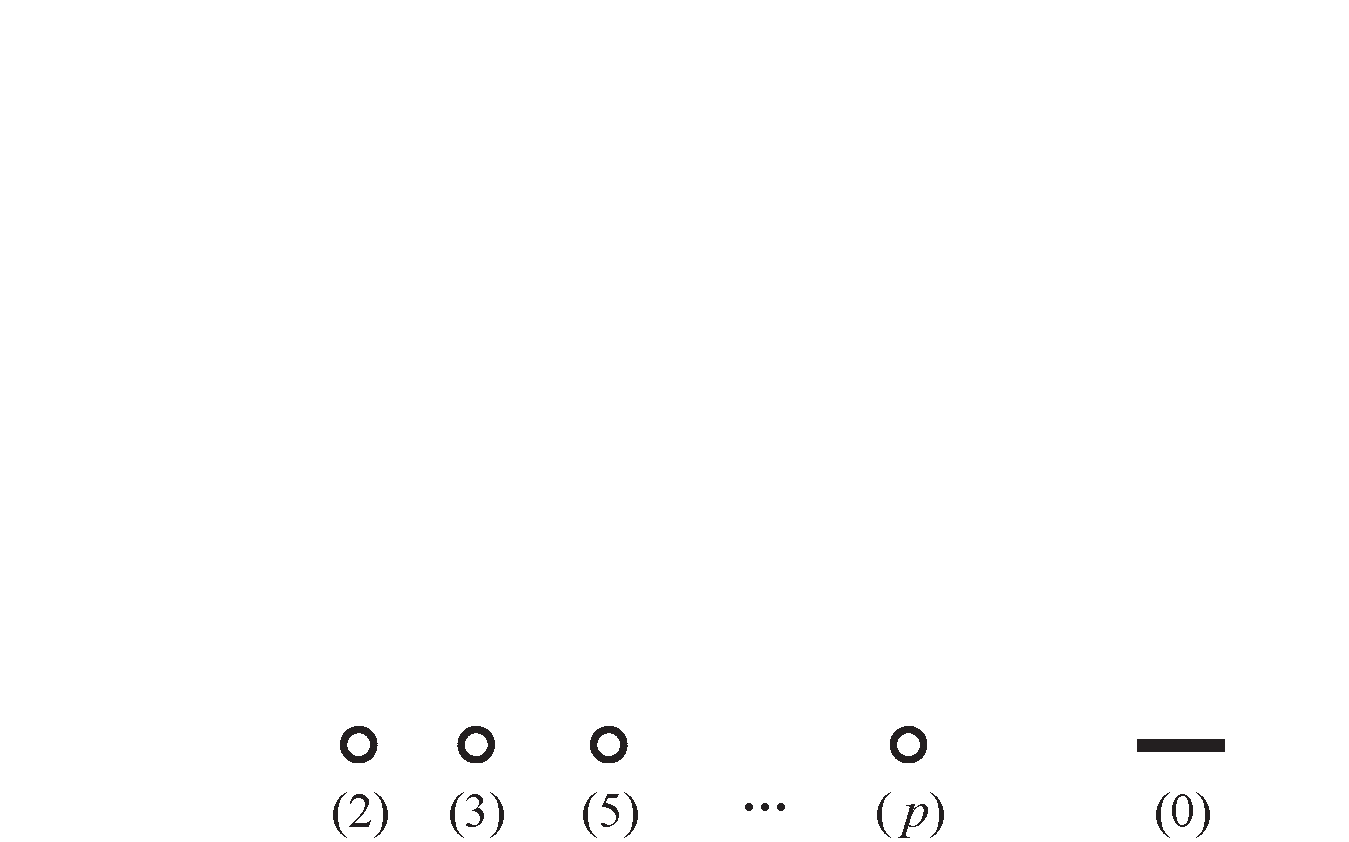
\includegraphics[width=4.25in]{SpecZ.pdf}
  \end{center}
  where the circles are closed points and zero has closure $\Spec\mathbf{Z}$. Now take $A = \mathbf{Z}$; then, by Problem $2.4$ we have that $\Hom_\Sch(X,\Spec\mathbf{Z}) \cong \Hom_\Rings(\mathbf{Z},\Gamma(X,\OO_X))$; however, since $\mathbf{Z}$ is the initial object in $\Rings$ \cite[Prop.~11.3.10]{Art11}, the latter set has one element and so there is a unique morphism $X\to\Spec\mathbf{Z}$, i.e., $\Spec\mathbf{Z}$ is the final object in $\Sch$.
\end{proof}

\begin{problem}
  Describe the spectrum of the zero ring, and show that it is an initial object for the category of schemes. (According to our conventions, all ring homomorphisms must take $1$ to $1$. Since $0=1$ is the zero ring, we see that each ring $R$ admits a unique homomorphism to the zero ring, but that there is no homomorphism from the zero ring to $R$ unless $0 = 1$ in $R$.)
\end{problem}
\begin{proof}
  The spectrum of the zero ring is the empty set with the trivial sheaf $\OO_{\Spec 0}(\emptyset) = 0$. Any scheme $(X,\OO_X)$ thus has a unique morphism defined by the morphism $\emptyset \to X$ on topological spaces and the morphism $\OO_X(U) \to 0$ on sections.
\end{proof}

\begin{problem}
  Let $X$ be a scheme. For any $x \in X$, let $\OO_x$ be the local ring at $x$, and $\mathfrak{m}_x$ its maximal ideal. We define the \emph{residue field} of $x$ on $X$ to be the field $k(x) = \OO_x/\mathfrak{m}_x$. Now let $K$ be any field. Show that to give a morphism of $\Spec K$ to $X$ it is equivalent to give a point $x \in X$ and an inclusion map $k(x) \to K$.
\end{problem}
\begin{proof}
  Suppose $\varphi\colon\Spec K \to X$ is a morphism of schemes; then, since $\Spec K = \{(0)\}$, the corresponding map on topological spaces is uniquely determined by the image of $(0)$ in $X$; call this $x$. Then, from $\varphi^\#$, taking the stalk at $x$ we obtain a map $\varphi^\#_x\colon \OO_x \to \OO_{\Spec K,(0)} = K$; since the map on rings is local, we have the map on residue fields
  \begin{equation*}
    \overline{\varphi^\#_x} \colon k(x) = \frac{\OO_x}{\mathfrak{m}_x} \to \frac{\OO_{\Spec K,(0)}}{(0)} = K,
  \end{equation*}
  which is injective since it is a ring homomorphism of fields.
  \par Now suppose we have a point $x \in X$ and an inclusion map $\iota\colon k(x) \to K$. As before, we can construct the map $\varphi\colon\Spec K \to X$ of topological spaces as $(0) \mapsto x$; it suffices to construct $\varphi^\#$. But we can let it be the composition
  \begin{equation*}
    \varphi^\#(U)\colon \OO_X(U) \to \OO_x \to \frac{\OO_x}{\mathfrak{m}_x} = k(x) \overset{\iota}{\longrightarrow} K = \OO_{\Spec K}(\Spec K),
  \end{equation*}
  when $U \ni x$, and $\varphi^\#(U) \equiv 0$ otherwise.
\end{proof}

\begin{problem}
  Let $X$ be a scheme. For any point $x \in X$, we define the \emph{Zariski tangent space} $T_x$ to $X$ at $x$ to be the dual of the $k(x)$-vector space $\mathfrak{m}_x/\mathfrak{m}_x^2$. Now assume that $X$ is a scheme over a field $k$, and let $k[\varepsilon]/\varepsilon^2$ be the \emph{ring of dual numbers} over $k$. Show that to give a $k$-morphism of $\Spec k[\varepsilon]/\varepsilon^2$ to $X$ is equivalent to giving a point $x \in X$, \emph{rational over $k$} (i.e., such that $k(x) = k$), and an element of $T_x$.
\end{problem}
\begin{proof}
  Suppose we have a $k$-morphism $\varphi\colon\Spec k[\varepsilon]/\varepsilon^2 \to X$. Note that $\Spec k[\varepsilon]/\varepsilon^2$ $= \{(\varepsilon)\}$ as a topological space; let $x = \varphi((\varepsilon))$. Since $\varphi$ is a $k$-morphism, we have the commutative diagrams
  \begin{equation*}
    \begin{tikzcd}[column sep=tiny]
      \Spec \frac{k[\varepsilon]}{\varepsilon^2} \arrow{rr}{\varphi}\arrow{dr} & & X\arrow{dl}\\
      & \Spec k
    \end{tikzcd} \overset{\text{stalks}}{\implies} 
    \begin{tikzcd}[column sep=tiny]
      \frac{k[\varepsilon]}{\varepsilon^2} \arrow[leftarrow]{rr}{\varphi^\#_{(\varepsilon)}}\arrow[leftarrow]{dr} & & \OO_x\arrow[leftarrow]{dl}\\
      & k
    \end{tikzcd} \overset{\text{residues}}{\implies} \begin{tikzcd}[column sep=tiny]
      k \arrow[leftarrow]{rr}{\varphi^\#_{(\varepsilon)}}\arrow[leftarrow]{dr} & & k(x)\arrow[leftarrow]{dl}\\
      & k
    \end{tikzcd}
  \end{equation*}
  Since our morphisms on stalks are local, we see that the maps on the right are all injections, hence $k(x) = k$ and $x$ is rational over $k$. Now note in the middle diagram that $\varphi^\#_{(\varepsilon)}(\mathfrak{m}_x) \subseteq (\varepsilon) \subseteq k[\varepsilon]/\varepsilon^2$, but $(\varepsilon^2) = 0$ implies that $\varphi^\#_{(\varepsilon)}(\mathfrak{m}_x^2) \subseteq (\varepsilon^2) = 0$. Thus, we get a map $\overline{\varphi^\#_{(\varepsilon)}} \in \Hom(\mathfrak{m}_x/\mathfrak{m}_x^2,k) = T_x$ by the universal property of the quotient, since $(\varepsilon) \cong k$ as vector spaces.
  \par In the other direction, suppose we have $x \in X$ rational over $k$ and an element $f \in T_x = \Hom(\mathfrak{m}_x/\mathfrak{m}_x^2,k)$. We construct the map $\varphi\colon\Spec k[\varepsilon]/\varepsilon^2 \to X$ to be the map $(\epsilon) \mapsto x$. Then, for $\varphi^\#$ we first consider when $U \ni x$. Then, since $x$ is a rational point $\OO_x \cong k \oplus \mathfrak{m}_x$, and so we can define the map
  \begin{equation*}
    \psi\colon k \oplus \mathfrak{m}_x \to \frac{k[\varepsilon]}{\varepsilon^2}, \quad (a,b) \mapsto a + f(b)\varepsilon.
  \end{equation*}
  Then, we can define $\varphi^\#(U)$ to be the composition
  \begin{equation*}
    \varphi^\#(U)\colon \OO_X(U) \to \OO_x \cong k \oplus \mathfrak{m}_x \overset{\psi}{\longrightarrow} \frac{k[\varepsilon]}{\varepsilon^2} = \varphi_*(\OO_{\Spec k[\varepsilon]/\varepsilon^2})(U).\qedhere
  \end{equation*}
\end{proof}

\begin{problem}
  If $X$ is a topological space, and $Z$ is an irreducible closed subset of $X$, a \emph{generic point} for $Z$ is a point $\zeta$ such that $Z = \{\zeta\}^-$. If $X$ is a scheme, show that every (nonempty) irreducible closed subset has a unique generic point.
\end{problem}
\begin{proof}
  Let $o(Z)$ denote the intersection of all non-empty open subsets of $Z$; $o(Z) \ne \emptyset$ since otherwise, there exist two disjoint open subsets $U_1,U_2$ of $Z$, and $Z = U_1^c \cup U_2^c$ contradicts irreducibility. Any point $x \in o(Z)$ is generic since if $x \in o(Z)$ is not, $U = X \setminus \overline{\{x\}} \ne \emptyset$ is open, contradicting the definition of $o(Z)$. Now suppose $y \ne x$ is another generic point of $Z$. Then, since the Zariski topology is $T_0$, there exists $U \ni x$ open such that $U \not\ni y$; then, $A = Z \setminus U$ is a closed proper subset of $Z$ which contains $y$, and so $\overline{\{y\}} \subseteq A \subsetneq Z$, i.e., $y$ cannot be a generic point.
\end{proof}

\begin{problem}
  Describe $\Spec \mathbf{R}[x]$. How does its topological space compare to the set $\mathbf{R}$? To $\mathbf{C}$?
\end{problem}
\begin{proof}[Solution]
  $\mathbf{R}[x]$ is a PID so all irreducibles are prime; thus, $\Spec \mathbf{R}[x]$ consists of prime ideals generated by irreducible polynomials and the generic point $(0)$. These prime ideals are closed, and are of the form $(x-\alpha)$ for $\alpha \in \mathbf{R}$ and $(x-\beta)(x-\overline{\beta})$ for $\beta \in \mathbf{C} \setminus \mathbf{R}$.
  \par We have the following maps of sets:
  \begin{equation*}
    \begin{tikzcd}[row sep=0em]
      \mathbf{R} \rar & \mathbf{C} \rar & \Spec\mathbf{R}[x]\\
      \alpha \arrow[mapsto]{rr} & & (x-\alpha)\\
      & \beta \arrow[mapsto]{r} & (x-\beta)(x-\overline{\beta})
    \end{tikzcd}
  \end{equation*}
  where the map $\mathbf{C} \to \Spec\mathbf{R}[x]$ is defined as for $\mathbf{R}$ when $\beta \in \mathbf{R}$. Then, $\mathbf{R} \hookrightarrow \Spec \mathbf{R}[x]$ is an injection, but the image of $\mathbf{R}$ is neither open nor closed, and does not have a generic point. The map from $\mathbf{C}$ is generically two-to-one on the image, but again, the image is neither open nor closed.
\end{proof}

\begin{problem}
  Let $k = \mathbf{F}_p$ be the finite field with $p$ elements. Describe $\Spec k[x]$. What are the residue fields of its points? How many points are there with a given residue field?
\end{problem}
\begin{proof}[Solution]
  Again, $\Spec k[x]$ consists of prime ideals generated by irreducible polynomials with the generic point $(0)$; note these are also maximal hence closed. The residue field at $(0)$ is the rational function field over $k$. If a maximal ideal is generated by a polynomial of degree $d$, then $k(x) = \mathbf{F}_{p^d}$. Finally, the number of irreducible polynomials of a given degree $d$, hence the number of points with a given residue field, is given by the M\"obius inversion formula \cite[p.~588]{DF04}:
  \begin{equation*}
    \psi(d) = \frac{1}{d} \sum_{\ell \mid d} \mu(\ell)p^{d/\ell},
  \end{equation*}
  where
  \begin{equation*}
    \mu(\ell) = \begin{cases}
      1 & \text{if}~\ell = 1,\\
      0 & \text{if $\ell$ has a square factor},\\
      (-1)^r & \text{if $\ell$ has $r$ distinct prime factors}.
    \end{cases}\qedhere
  \end{equation*}
\end{proof}

\begin{problem}
  \emph{Glueing Lemma}. Generalize the glueing procedure described in the text $(2.3.5)$ as follows. Let $\{X_i\}$ be a family of schemes (possibly infinite). For each $i \ne j$, suppose given an open subset $U_{ij} \subseteq X_i$, and let it have the induced scheme structure $(\mathrm{Ex}.~2.2)$. Suppose also given for each $i \ne j$ an isomorphism of schemes $\varphi_{ij}\colon U_{ij} \to U_{ji}$ such that $(1)$ for each $i,j$, $\varphi_{ji} = \varphi_{ij}^{-1}$, and $(2)$ for each $i,j,k$, $\varphi_{ij}(U_{ij} \cap U_{ik}) = U_{ji} \cap U_{jk}$, and $\varphi_{ij} = \varphi_{jk} \circ \varphi_{ij}$ on $U_{ij} \cap U_{ik}$. Then show that there is a scheme $X$, together with morphisms $\psi_i\colon X_i \to X$ for each $i$, such that $(1)$ $\psi_i$ is an isomorphism of $X_i$ onto an open subscheme of $X$, $(2)$ the $\psi_i(X_i)$ cover $X$, $(3)$ $\psi_i(U_{ij}) = \psi_i(X_i) \cap \psi_j(X_j)$ and $(4)$ $\psi_i = \psi_j \circ \varphi_{ij}$ on $U_{ij}$. We say that $X$ is obtained by \emph{glueing} the schemes $X_i$ along the isomorphisms $\varphi_{ij}$. An interesting special case is when the family $X_i$ is arbitrary, but the $U_{ij}$ and $\varphi_{ij}$ are all empty. Then the scheme $X$ is called the \emph{disjoint union} of the $X_i$, and is denoted $\coprod X_i$.
\end{problem}
\begin{proof}
  Define the topological space on $X$ to be
  \begin{equation*}
    X = \frac{\displaystyle\coprod X_i}{\varphi_{ij}(x) \sim x},
  \end{equation*}
  where the equivalence relation runs over all $x \in U_{ij}$ and all $i \ne j$, with the quotient topology; hypothesis $(1)$ ensures symmetry of our equivalence relation and $(2)$ ensures transitivity. Let $\psi_i\colon X_i \to X$ denote the equality above precomposed with the map $X_i \to \coprod X_i/\sim$. The $\psi_i(X_i)$ then form an open cover of $X$, proving $(2)$. By Problem $1.22$, we can glue the $\OO_{X_i}$ together to form a sheaf $\OO_X$ on $X$. This makes $X$ a scheme since for any $x \in X$, we can choose a neighborhood small enough that it is contained in a $X_i$, and $X_i$ is locally affine. The $\psi_i$ form morphisms just by the identity morphism on each part of $X$, proving $(1)$. $(3)$ follows by definition of the quotient space, as does $(4)$.
\end{proof}

\begin{problem}
  A topological space is \emph{quasi-compact} if every open cover has a finite subcover.
  \begin{enuma}
    \item Show that a topological space is noetherian $(\mathrm{I},\S1)$ if and only if every open subset is quasi-compact.
    \item If $X$ is an affine scheme, show that $\Sp(X)$ is quasi-compact, but not in general noetherian. We say a scheme $X$ is \emph{quasi-compact} if $\Sp(X)$ is.
    \item If $A$ is a noetherian ring, show that $\Sp(\Spec A)$ is a noetherian topological space.
    \item Give an example to show that $\Sp(\Spec A)$ can be noetherian even when $A$ is not.
  \end{enuma}
\end{problem}
\begin{proof}[Proof of $(a)$]
  Suppose our topological space $X$ is noetherian. Let $U \subseteq X$, and let $A_1 \supseteq A_2 \supseteq A_3 \supseteq \cdots$ be a descending chain of closed sets in $Y$; write $A_i = Y \cap V_i$ for $V_i \subseteq X$ closed. Then, $V_1 \supsetneq V_1 \cap V_2 \supsetneq V_1 \cap V_2 \cap V_3 \supsetneq \cdots$ stabilizes since $X$ is noetherian, and so $A_1 \supseteq A_2 \supseteq A_3 \supseteq \cdots$ does as well. Now suppose $Y = \bigcup_{\alpha \in A} Y_\alpha$ is an open covering of $Y$ that has no finite subcover. We construct $\alpha_i$ inductively as follows: if $Y \ne Y_{\alpha_1} \cup \cdots \cup Y_{\alpha_n}$, then choose $\alpha_{n+1}$ such that $Y_{\alpha_{n+1}} \not\subseteq Y_{\alpha_1} \cup \cdots Y_{\alpha_n}$. Then,
  \begin{equation*}
    Y \supsetneq (Y \setminus Y_{\alpha_1}) \supsetneq (Y \setminus (Y_{\alpha_1} \cup Y_{\alpha_2})) \supsetneq \cdots
  \end{equation*}
  is a strictly decreasing chain of closed sets that does not stabilize, contradicting that $Y$ is noetherian.
  \par Now suppose that $X$ is such that every open subset is quasi-compact. Let $U_1 \subseteq U_2 \subseteq \cdots$ be an ascending chain of open subsets of $X$. Then, $\bigcup U_i$ has a finite subcover by assumption, and so the chain must stabilize, i.e., $X$ is noetherian.
\end{proof}
\begin{proof}[Proof of $(b)$]
  Suppose $X = \Spec R$. Recall that the sets $D(f)$ for $f \in R$ form a basis of $X$, and so any open cover of $X$ has a refinement of the form $\bigcup X_{f_\alpha}$. Thus,
  \begin{align*}
    X = \bigcup_{\alpha \in A} X_{f_\alpha} &\iff 1 \in \braket{f_\alpha}_{\alpha \in A}\\
    &\iff 1 = h_1f_1 + \cdots + h_mf_m\\
    &\iff X = D(f_1) \cup \cdots \cup D(f_m),
  \end{align*}
  and $X$ is therefore quasicompact.
  \par Now suppose $X = \Spec k[x_1,x_2,\ldots]$. Then, $V(x_1) \supsetneq V(x_1,x_2) \supsetneq \cdots$ is a descending chain that does not stabilize.
\end{proof}
\begin{proof}[Proof of $(c)$]
  If $V(I_1) \supseteq V(I_2) \supseteq V(I_3) \supseteq \cdots$ is a descending chain, we have the corresponding ascending chain $\sqrt{I_1} \subseteq \sqrt{I_2} \subseteq \sqrt{I_3} \subseteq \cdots$ in $A$, which stabilizes since $A$ is noetherian; thus, the descending chain of closed sets also stabilizes.
\end{proof}
\begin{proof}[Proof of $(d)$]
  Let $A = k[x_1,x_2,\ldots]/(x_1^2,x_2^2,\ldots)$, and $X = \Spec A$. $X$ then consists of one point, $(x_1,x_2,\ldots)$, since this is the only prime ideal in $A$ (it is the only prime ideal that contains $(x_1^2,x_2^2,\ldots)$ in $k[x_1,x_2,\ldots]$), and so is trivially noetherian. The ring, however, is not noetherian since $(x_1) \subsetneq (x_1,x_2) \subsetneq \cdots$ is an ascending chain that does not stabilize.
\end{proof}

\begin{problem}\mbox{}
  \begin{enuma}
    \item Let $S$ be a graded ring. Show that $\Proj S = \emptyset$ if and only if every element of $S_+$ is nilpotent.
    \item Let $\varphi\colon S \to T$ be a graded homomorphism of graded rings (preserving degrees). Let $U = \{\mathfrak{p} \in \Proj T \vert \mathfrak{p} \not\supseteq \varphi(S_+)\}$. Show that $U$ is an open subset of $\Proj T$, and show that $\varphi$ determines a natural morphism $f \colon U \to \Proj S$.
    \item The morphism $f$ can be an isomorphism even when $\varphi$ is not. For example, suppose that $\varphi_d\colon S_d \to T_d$ is an isomorphism for all $d \ge d_0$, where $d_0$ is an integer. Then show that $U = \Proj T$ and the morphism $f \colon \Proj T \to \Proj S$ is an isomorphism.
    \item Let $V$ be a projective variety with homogeneous coordinate ring $S$ $(\mathrm{I},\S2)$. Show that $t(V) \cong \Proj S$.
  \end{enuma}
\end{problem}
\begin{proof}[Proof of $(a)$]
  $S_+ \subseteq \mathfrak{N}(S) \implies S_+ \subseteq \mathfrak{p}$ for all prime ideals $\mathfrak{p}$, and so $\Proj S = \emptyset$.
  \par Conversely, suppose $\Proj S = \emptyset$, and consider $f \in S_+$ homogeneous. Then, $D(f) = \emptyset \implies \Spec S_{(f)} = \emptyset$. Thus, $S_{(f)} = 0$, and so $1/f^n = 0$, and $f^n = 0$ for some $n$, i.e., $f$ is nilpotent. Homogeneous elements generate $S_+$ so $S_+ \subseteq \mathfrak{N}(S)$.
\end{proof}
\begin{proof}[Proof of $(b)$]
  $\varphi(S_+)$ is a homogeneous ideal, and so $U^c = \{\mathfrak{p} \in \Proj T \vert \mathfrak{p} \supseteq \varphi(S_+)\}$ is closed.
  \par Now $\varphi$ determines a natural morphism $f\colon U \to \Proj S$ by $f(x) = \varphi^{-1}(x)$. This is continuous since $f^{-1}(V(I)) = V(\varphi(I))$. We then define the sheaf morphism $f^\#\colon \OO_S(V) \to \OO_T(f^{-1}(V))$ for $V \subseteq \Proj S$ by composing a section $s\colon V \to \coprod S_{\varphi^{-1}(\mathfrak{p})}$ where the $\mathfrak{p}\in V$, with the morphisms $\varphi_{(\mathfrak{p})}\colon S_{\varphi^{-1}(\mathfrak{p})} \to T_{\mathfrak{p}}$.
\end{proof}
\begin{proof}[Proof of $(c)$]
  Let $\mathfrak{p} \in \Proj T$; choose $t \in T_+ \setminus \mathfrak{p}$. $\deg t \ge 1$, and so $\deg t^k \ge d_0$ for some $k$. Since $\varphi_d$ is an isomorphism for all $d \ge d_0$, there exists $s \in S_+$ such that $\varphi(s) = t^k \notin \mathfrak{p}$, and so $\varphi(S_+) \not\subseteq \mathfrak{p}$. Thus, $\mathfrak{p} \in U$, and so $U = \Proj T$.
  \par Now choose $t_i$ that generate $T_+$. Then, $\bigcup D_+(t_i) = \Proj T$ forms an open cover; similarly, $\bigcup D_+(t_i^{d_0}) = \Proj T$. Since we can find $s_i$ such that $\varphi(s_i) = t_i^{d_0}$ by the fact that $\varphi$ is an isomorphism for $d \ge d_0$. We then have a morphism of affine schemes $f_i\colon D(t_i) \to D(s_i)$ induced by the restriction of $f$; to show $f$ is an isomorphism, it then suffices to show that each $f_i$ is an isomorphism, for gluing is immediate since we are just taking restrictions of $f$. We note $\cup D(s_i) = \Proj S$, for if not, and $\mathfrak{p} \ni s_i$ for every $i$, then $f(\mathfrak{p}) \ni t_i$ for all $i$, i.e., $f(\mathfrak{p}) \supseteq T_+$.
  \par Now to see that $f$ is injective, it suffices to show injectivity on each $i$. Suppose $f/s^n \mapsto 0$; then, $0 = t^m\varphi(f) = \varphi(s^m)\varphi(f)$ for some $m$. Thus, $s^mf \in \ker\varphi$. Exponentiating by a power large enough makes $s^mf \in S_d$ which is isomorphic to $T_d$; thus, $s^mf = 0$ and $f/s^m = 0$, and so $f$ is injective. Now if $f/t^n \in T_{(t)}$, this is equal to $t^{d_0}f/t^{n+d_0}$; but then, $t^{d_0}f$ has high enough degree such that it has preimage in $S$; our morphism is therefore surjective as well.
\end{proof}
\begin{proof}[Proof of $(d)$]
  Recall $t(V)$ is the set of all (nonempty) irreducible closed subsets of $V$; these are defined by $I$ homogeneous ideals not equal to $S_+$, and so the map $f$ sending an irreducible closed subset of $V$ defined by an ideal $I$ to $V(I)$ of its associated ideal is a bijection by Exercise I.2.4. Now, recall the closed sets of $t(V)$ are of the form $t(W)$ for $W$ closed in $V$; to check continuity, it suffices to check continuity for basis elements. But the preimage of $D_+(f)$ for any $f$ is still open by definition of $t(V)$, and similarly the image of any (closed) basis element $t(W)$ for $W$ defined by $I$ closed in $V$ is the ideal $\sqrt{I}$, which is still closed.
  \par We claim that we have an isomorphism on sheaves. Recall that the sheaf is given by $(t(V),\alpha_*(\OO_V))$. We then want to define $f^\#\colon \OO_{\Proj S}(U) \to f_*\OO_{t(V)}(U) = \OO_{V}(\alpha^{-1}(f^{-1}(U)))$. But this works since local sections on one side uniquely determine local sections on the other.
\end{proof}

\begin{problem}\mbox{}
  \begin{enuma}
    \item Let $V$ be a variety over the algebraically closed field $k$. Show that a point $P \in t(V)$ is a closed point if and only if its residue field is $k$.
    \item If $f\colon X \to Y$ is a morphism of schemes over $k$, and if $P \in X$ is a point with residue field $k$, then $f(P) \in Y$ also has residue field $k$.
    \item Now show that if $V,W$ are any two varieties over $k$, then the natural map
      \begin{equation*}
        \Hom_{\Var}(V,W) \to \Hom_{Sch/k}(t(V),t(W))
      \end{equation*}
      is bijective. (Injectivity is easy. The hard part is to show it is surjective.)
  \end{enuma}
\end{problem}
\begin{proof}[Proof of $(a)$]
  Suppose $P \in t(V)$ with $k(P) = k$. Then $P$ corresponds to a maximal ideal $\mathfrak{m}_i$ in each affine chart $\Spec A_i$ since a subset of $t(V)$ is closed if and only if its restriction is closed in every affine chart; thus it is itself a closed point.
  \par Now suppose $P$ is a closed point; then, it is closed in some open affine chart $\Spec A$. There, $P$ is a maximal ideal, and so $k(P) = \OO_{X,P}/\mathfrak{m}_P = k$.
\end{proof}
\begin{proof}[Proof of $(b)$]
  Since $f$ is a $k$-morphism, we have the commutative diagrams
  \begin{equation*}
    \begin{tikzcd}[column sep=tiny]
      X \arrow{rr}{f}\arrow{dr} & & Y\arrow{dl}\\
      & \Spec k
    \end{tikzcd} \overset{\text{stalks and residue}}{\implies} 
    \begin{tikzcd}[column sep=tiny]
      k \arrow[leftarrow]{rr}{f^\#_{(P)}}\arrow[leftarrow]{dr} & & k(P)\arrow[leftarrow]{dl}\\
      & k
    \end{tikzcd}
  \end{equation*}
  Since our morphisms on stalks are local, we see that the maps on the right are all injections, hence $k(P) = k$.
\end{proof}
\begin{proof}[Proof of $(c)$]
  Define the map by having $\varphi\colon V \to W$ map to the extension of $\overline{\varphi}$ onto all of $t(V)$ by mapping an irreducible closed subset to the closure of its image. Note that $P$ closed maps to $\overline{\varphi}(P)$ closed as well by $(b)$. This implies injectivity, since $\varphi \ne \psi$ implies they act differently on some point $P \in V$, and so their extensions will as well.
  \par Now, for surjectivity, suppose $\psi\colon t(V) \to t(W)$. We claim that $\varphi = \psi\vert_V$ maps to $\psi$; this is clear since continuous maps were defined such that $\psi(P) = \overline{\{P\}}$ in the first place, and by $(b)$ closed points are mapped to closed points. It therefore suffices to show $\psi$ is regular. Let $U \subseteq W$ be an affine chart; it has preimage $\psi^{-1}(U)$; restricting as necessary we can assume we have $V \supset U' \to U \subset W$ a map between affine charts. But recall that regular maps are given uniquely by maps between rings of sections by Prop.~I.3.5; in our case, we have the ring maps given by the ring maps on sections between $\OO_{t(W)}(U) \to \OO_{t(V)}(U')$, and so we are done.
\end{proof}

\begin{problem}
  Let $X$ be a scheme, and let $f \in \Gamma(X,\OO_X)$, and define $X_f$ to be the subset of points $x \in X$ such that the stalk $f_x$ of $f$ at $x$ is not contained in the maximal ideal $\mathfrak{m}_x$ of the local ring $\OO_x$.
  \begin{enuma}
    \item If $U = \Spec B$ is an open \emph{affine} subscheme of $X$, and if $\overline{f} \in B = \Gamma(U,\OO_X\vert_U)$ is the restriction of $f$, show that $U \cap X_f = D(\overline{f})$. Conclude that $X_f$ is an open subset of $X$.
    \item Assume that $X$ is quasi-compact. Let $A = \Gamma(X,\OO_X)$, and let $a \in A$ be an element whose restriction to $X_f$ is $0$. Show that for some $n > 0$, $f^na = 0$.
    \item Now assume that $X$ has a finite cover by open affines $U_i$ such that each intersection $U_i \cap U_j$ is quasi-compact. (This hypothesis is satisfied, for example, if $\Sp(X)$ is noetherian.) Let $b \in \Gamma(X_f,\OO_{X_f})$. Show that for some $n > 0$, $f^nb$ is the restriction of an element of $A$.
    \item With the hypothesis of $(c)$, conclude that $\Gamma(X_f,\OO_f) \cong A_f$.
  \end{enuma}
\end{problem}
\begin{proof}[Proof of $(a)$]
  Suppose $x \in U \cap X_f$; then, since $x = \mathfrak{p}$ for some prime in $B$, $f_x \notin \mathfrak{m}_x \iff \overline{f} \notin \mathfrak{p} \iff x \in D(\overline{f})$, since by the definition of stalk $f_x = \overline{f}_x$. Now since we can cover $X_f$ with open sets, it is open.
\end{proof}
\begin{proof}[Proof of $(b)$]
  Since $X$ is quasi-compact, it has a finite affine covering. Now in each affine chart $U_i = \Spec B_i$, $U_i \cap X_f = D(\overline{f})$ by $(a)$. Since $a \in A$ restricts to $0$ in $X_f$, its restriction to $D(\overline{f})$ is $0$ as well. Noting $\OO_X(D(\overline{f})) = \OO_{U_i}(D(\overline{f})) = (B_i)_{\overline{f}}$ by Proposition $2.2(b)$. Thus, there exists some $n_i$ such that $\overline{f}{}^{n_i}a = 0$, and so taking the maximum $n$ of these $n_i$ over the (finite) affine cover, we see that $f^na = 0$ when restricting to each $U$. By the sheaf property, $f^na = 0$.
\end{proof}
\begin{proof}[Proof of $(c)$]
  Let $U_i = \Spec B_i$; $b$ then has image
  \begin{equation*}
    \frac{b_i}{f_i^{n_i}} \in \OO_X(U_i \cap X_f) = \OO_{\Spec B_i}(D(f_i)) = (B_i)_{f_i}
  \end{equation*}
  by $(a)$, where $f_i$ is the image of $f$ in $\OO_X(U_i)$. Multiplying $b$ by $f^n$ where $n = \max n_i$ gives that $bf^n \in \OO_X(X_f)$ has image $b_if_i^{n-n_i}/1 \in \OO_{\Spec B_i}(D(f_i))$, which lifts to $b_if_i^{n-n_i} \in \Spec B_i$. We now claim that these $b_if_i^{n-n_i}$ lift to some element in $\OO_X(X) = A$. But this is true since on each intersection $(U_i \cap U_j) \cap X_f$, the restrictions satisfy $b_if_{ij}^{n-n_i} - b_jf_{ji}^{n-n_j} = 0$ and so by $(b)$, $f_{ij}^{m_{ij}}(b_if_{ij}^{n-n_i} - b_jf_{ij}^{n-n_j}) = 0$ for some $m_{ij}$. Taking $m = \max m_{ij}$, gluing these sections $b_if_i^{m+n-n_i}$ together produces the element in $A$ we require.
\end{proof}
\begin{proof}[Proof of $(d)$]
  Define the map $\Gamma(X_f,\OO_f) \to A_f$ by mapping $b \mapsto a/f^n$, where $a$ is the element in $(c)$ that restricts to $bf^n$ on $X_f$. This is well defined since if $bf^m$ lifted to $a' \in A$, then assuming without loss of generality $m > n$, the restriction of $f^{n}(f^{m-n}a'-a)$ is zero, and then applying $(b)$. This map is injective since if $b$ was such that $bf^n$ had lift $a$, and $b'$ was such that $b'f^m$ had lift $a'$, then $a/f^n = a'/f^m \implies b = b'$. This map is surjective since if $a/f^n \in A_f$, then $\overline{a} \in b$ lifts to $a$, and so $\overline{a}/\overline{f}^n \mapsto a/f^n$.
\end{proof}

\begin{problem}
  \emph{A Criterion for Affineness}.
  \begin{enuma}
  \item Let $f\colon X \to Y$ be a morphism of schemes, and suppose that $Y$ can be covered by open subsets $U_i$, such that for each $i$, the induced map $f^{-1}(U_i) \to U_i$ is an isomorphism. Then $f$ is an isomorphism.
  \item A scheme $X$ is affine if and only if there is a finite set of elements $f_1,\ldots,f_r \in A = \Gamma(X,\OO_X)$, such that the open subsets $X_{f_i}$ are affine, and $f_1,\ldots,f_r$ generate the unit ideal in $A$.
  \end{enuma}
\end{problem}
\begin{proof}[Proof of $(a)$]
  We first show $f$ is a homeomorphism on topological spaces. If $W \subseteq Y$, then $f^{-1}(W) = \bigcup f^{-1}(W \cap U_i)$ is open, and if $V \subseteq X$, then $f(V) = \bigcup f(V \cap f^{-1}(U_1))$ is open, and so it remains to show $f$ is bijective. $f$ is surjective since very $y \in Y$ is in particular in some $U_i$, and so it has a preimage in $f^{-1}(U_i) \subseteq X$; likewise, $f$ is injective since if $f(x) = f(y) \in U_i$ for some $i$, then they must have the same preimage in $f^{-1}(U_i)$.
  \par Now it remains to show that we have an isomorphism of sheaves. But this is true since we have an isomorphism on stalks by Prop.~1.1.
\end{proof}
\begin{proof}[Proof of $(b)$]
  If $A$ is affine, then we can take $f_1 = 1$ and be done. In the other direction, we have a morphism of commutative rings $A \to \Gamma(X,\OO_X)$, and so we automatically have a morphism of schemes $\varphi\colon X \to \Spec A$ by Problem $2.4$; we want to show this is an isomorphism.
  %We first have the morphisms of commutative rings
  %\begin{equation*}
  %  \begin{tikzcd}
  %    A \rar{\id} \dar & \Gamma(X,\OO_X) \dar \rar[equals] & A \dar\\
  %    A_{f_i} & \Gamma(X_{f_i},\OO_{X_{f_i}}) \rar[equals] & A_{f_i}
  %  \end{tikzcd}
  %\end{equation*}
  %where the vertical maps are the localization. Applying Problem $2.4$ gives the morphisms of schemes
  %\begin{equation*}
  %  \begin{tikzcd}
  %    X \rar & \Spec A\\
  %    X_{f_i} \uar[hookrightarrow] & D(f_i) \uar[hookrightarrow]
  %  \end{tikzcd}
  %\end{equation*}
  Since $\braket{f_1,\ldots,f_r} = A$, $\Spec A = D(f_1) \cup \cdots \cup D(f_r)$ is an open cover. The preimage of each $D(f_i)$ is $X_{f_i}$ by construction of the map $X \to \Spec A$ in Problem $2.4$. To show our claim, it suffices to show that $\varphi_i \coloneqq \varphi\vert_{X_{f_i}}\colon X_{f_i} \to D(f_i)$ is an isomorphism; it suffices to show we have an isomorphism $A_{f_i} \to \Gamma(X_{f_i},\OO_X)$ of rings since both $X_{f_i}$ and $D(f_i) = \Spec A_{f_i}$ are affine. For injectivity, suppose $a/f_i^n \mapsto 0$; then, it vanishes in each $X_i \cap X_j = \Spec(A_{f_j})_{f_i}$, so for each $j$ there is some $n_j$ such that $a/f_j^{n_j} = 0$ in $A_{f_j}$. Letting $m = \max n_j$ means that $f_i^ma = 0$ and so $a/f_i^n = 0$ in $A_{f_i}$. For surjectivity, let $a \in A_{f_i} = \Gamma(X_{f_i},\OO_X)$ by Problem $2.16d$. Then, $a\vert_{X_{f_i,f_j}} = b_j/f_j^{n_j}$ for some $b_j \in A_{f_j}$ and $n_j \in \mathbf{N}$. So, for some $n$ large enough, we have an element $b_j \in A_{f_j}$ such that its restriction on each $X_{f_if_j}$ is $f_i^{n}a$. On triple intersections $X_{f_if_jf_k}$ we have $b_j - b_k = f_i^na - f_i^na = 0$ and so there exists $m_{jk}$ such that $f_i^{m_{jk}}(b_j-b_k) = 0$. Replacing them all with large enough $m$, we have $f_i^mb_j$ for each $X_{f_j}$, and together with $f_i^{n+m}a$ on $X_{f_i}$ we have sections that all agree on intersections. By the sheaf property, we then have a global section $s$ which restricts to $f_i^{n+m}a$ on $X_{f_i}$, and so $s/f_i^{n+m} \mapsto a$ by $\varphi\vert_{X_{f_i}}$.
  \par Finally, by $(a)$ of this problem we are done.
\end{proof}

\begin{problem}
  In this exercise, we compare some properties of a ring homomorphism to the induced morphism of the spectra of the rings.
  \begin{enuma}
    \item Let $A$ be a ring, $X = \Spec A$, and $f \in A$. Show that $f$ is nilpotent if and only if $D(f)$ is empty.
    \item Let $\varphi\colon A \to B$ be a homomorphism of rings, and let $f\colon Y = \Spec B \to X = \Spec A$ be the induced morphism of affine schemes. Show that $\varphi$ is injective if and only if the map of sheaves $f^\#\colon \OO_X \to f_*\OO_Y$ is injective. Show furthermore in that case $f$ is \emph{dominant,} i.e., $f(Y)$ is dense in $X$.
    \item With the same notation, show that if $\varphi$ is surjective, then $f$ is a homeomorphism of $Y$ onto a closed subset of $X$, and $f^\#\colon \OO_X \to f_*\OO_Y$ is surjective.
    \item Prove the converse to $(c)$, namely, if $f\colon Y \to X$ is a homeomorphism onto a closed subset, and $f^\#\colon\OO_X \to f_*\OO_Y$ is surjective, then $\varphi$ is surjective.
  \end{enuma}
\end{problem}
\begin{proof}[Proof of $(a)$]
  $f \in \mathfrak{N}(A) = \bigcap \mathfrak{p}$, where $\mathfrak{p}$ ranges over all prime ideals of $A$ $\iff f \in \mathfrak{p}$ for all $\mathfrak{p} \in \Spec A \iff D(f) = \emptyset$.
\end{proof}
\begin{proof}[Proof of $(b)$]
  If $f^\#$ is injective, then it is injective for $f^\#(X) = \varphi$. Conversely, suppose $\varphi$ is injective. It suffices to show that the map $f_\mathfrak{p}\colon \OO_{\Spec A,\mathfrak{p}} \to f_*\OO_{\Spec B,\mathfrak{p}}$ is injective. We note that, letting $S = \varphi(A \setminus \mathfrak{p})$,
  \begin{align*}
    f_*\OO_{\Spec B,\mathfrak{p}} &= \varinjlim_{U \ni \mathfrak{p}} \OO_{\Spec B}(f^{-1}(U))\\
    &= \varinjlim_{D(a) \ni \mathfrak{p}} \OO_{\Spec B}(f^{-1}(D(a)))\\
    &= \varinjlim_{D(\varphi(a)) \ni \varphi(\mathfrak{p})} \OO_{\Spec B}(D(\varphi(a)))\\
    &= S^{-1}B
  \end{align*}
  where the second line follows since $D(a)$ for $a \in A$ form a basis, and the third line follows since $D(a) \ni \mathfrak{p} \iff a \notin \mathfrak{p} \implies \varphi(a) \notin \varphi(\mathfrak{p})$; the last line is just by definition of the direct limit, since $S = \varphi(A \setminus \mathfrak{p}) = \{\varphi(a) \vert \varphi(\mathfrak{p}) \in D(\varphi(a)) \}$. We note that by \cite[Prop.~3.5]{AM69}, we have that $S^{-1}B \cong B \otimes_A A_\mathfrak{p}$. Injectivity of the map $A \to B$ then ensures $A_\mathfrak{p} \to S^{-1}B \cong B \otimes_A A_\mathfrak{p}$ is also injective by the exactness of direct limits \cite[Ex.~2.19]{AM69}.
  \par To show it is dominant, we consider $W \coloneqq X \setminus \overline{f(Y)}$; suppose $W \ne \emptyset$. $W$ is then covered by basis elements of the form $D(f)$, where $f \in \varphi^{-1}\mathfrak{p}$ for all $\mathfrak{p} \in \Spec B$. But then, $\varphi(f) \in \mathfrak{p}$ for all $\mathfrak{p} \in \Spec B$, and so $\varphi(f)$ is nilpotent; thus, $f$ is also nilpotent by injectivity of $\varphi$ and we have $D(f) = \emptyset$ by $(a)$.
\end{proof}
\begin{proof}[Proof of $(c)$]
  Now suppose $\varphi$ is surjective; this induces an isomorphism $A/\ker\varphi \cong B$, and so we immediately have a bijection between primes containing $\ker\varphi$ in $A$ and primes in $B$. We claim this is a homeomorphism $\Spec B \to V(\ker\varphi) \subset \Spec A$; since the induced map on topological spaces is automatically continuous, it suffices to show it is closed. But this is true since a basis element $D(f) \subset \Spec B$ maps to $D(\varphi^{-1}(f))$ in $\Spec A$, whose intersection with $V(\ker\varphi)$ is also open by definition of the induced topology on $V(\ker\varphi)$. The map $f^\#$ is clearly surjective since it induces the map $A_\mathfrak{p} \to B \otimes_A A_\mathfrak{p}$ on stalks, which is surjective by the right exactness of the tensor product.
\end{proof}
\begin{proof}[Proof of $(d)$]
  Since $f^\#$ is surjective, it is surjective on every stalk, i.e., the maps $A_{\mathfrak{p}} \to B \otimes_A A_\mathfrak{p}$ are surjective for all $\mathfrak{p}$. But $A \to B$ is surjective if and only if $A_{\mathfrak{p}} \to B \otimes_A A_\mathfrak{p}$ is surjective for all prime $\mathfrak{p}$ by \cite[Prop.~3.9]{AM69}.
\end{proof}

\begin{problem}
  Let $A$ be a ring. Show that the following conditions are equivalent:
  \begin{enumi}
    \item $\Spec A$ is disconnected;
    \item there exist nonzero elements $e_1,e_2 \in A$ such that $e_1e_2 = 0$, $e_1^2 = e_1$, $e_2^2 = e_2$, $e_1 + e_2 = 1$ (these elements are called \emph{orthogonal idempotents});
    \item $A$ is isomorphic to a direct product $A_1 \times A_2$ of two nonzero rings.
  \end{enumi}
\end{problem}
\begin{proof}
  $(i) \Rightarrow (ii)$. Say $\Spec A = U_1 \amalg U_2$. These are also closed, so $U_1 = V(I_1)$, $U_2 = V(I_2)$. Then, $V(0) = X = U_1 \amalg U_2 = V(I_1\cdots I_2)$, and so $I_1I_2 \subset \sqrt{0}$. Likewise, $V(A) = \emptyset = U_1 \cap U_2 = V(I_1 + I_2)$, and so $\sqrt{I_1 + I_2} = R$. By \cite[Ex.~1.13iv]{AM69}, this implies $I_1 + I_2 = R$. Thus, $x_1 + x_2 = 1$ for some $x_1 \in I_1$, $x_2 \in I_2$.
  \par Now since $I_1I_2 \subset \sqrt{0}$, we have $(x_1x_2)^m = 0$ for some $m$. Then, we have
  \begin{equation*}
    1 = (x_1 + x_2)^{2m} = \underbrace{x_1^{2m} + \cdots + \binom{2m}{m+1} x_1^{m+1}x_2^{m-1}}_{e_1} + \underbrace{\binom{2m}{m}x_1^mx_2^m + \cdots + x_2^{2m}}_{e_2}
  \end{equation*}
  Then, we have $e_1e_2 = 0$, $e_1^2 = e_1$, and $e_2^2 = e_2$.
  \par $(ii) \Rightarrow (iii)$. We first see that $A = \braket{e_1} \oplus \braket{e_2} = A_1 \times A_2$ where $A_1 = \braket{e_1}$, $A_2 = \braket{e_2}$, for $e_1 + e_2 = 1$, and this is a direct product by the orthogonality relations.
  \par $(iii) \Rightarrow (i)$. If $A \cong A_1 \times A_2$, then letting $e_1$ be the generator of $A_1$ and $e_2$ the generator of $A_2$, we have $A_1 \cong A/\Ann_A e_1$ and $A_2 \cong A/\Ann_A e_2$; thus, we have the partition $\Spec A = V(\Ann_A e_1) \amalg V(\Ann_A e_2)$.
\end{proof}

\printbibliography
\end{document}
